\section{Performance results}
\label{section:results}

We study the behaviour of our algorithms at hands of an artificial granulate
setup. 
Granulates of various diameters between $diam_{min}$ and $diam_{max}$ are
randomly distributed in a unit cube.
They are assigned random velocity and fixed density. 
If particles bump into the unit cube wall, they are reflected by applying an opposite direction in the velocities. 
We apply a full elastic collision model by allowing virtual penetration using the DEM spring-dashpot penalty force function (\ref{xxx}).
Each particle is created by a randomised algorithm that places a random number
of 50 points within the unit sphere. 
We then use the hull algorithm \cite{xxxx} using a Delaunay triangulation to
create the particle that is finally shrinked to fit into the prescribed
diameter.
On average, we obtain around 60-65 triangles per non-spherical particle.


The underlying spacetree is based upon tree-partitioning as we rely on the AMR
framework Peano \cite{Software:Peano}.
All experiments are realised with double precision. 
We note that the combination of the present work with reduced
floating-point accuracy, notably following
\cite{Weinzierl:15:Compression}, however could be advantageous.
All particle velocities and time step sizes $ \Delta t$ are chosen reasonably
small such that particles do never penetrate or jump over more than one grid cell per time step.
Higher velocities require more sophisticated collision models and a more
sophisticated vertex association as discussed in \cite{Weinzierl:16:PIC}.
Particles are assumed to collide as soon as they get closer than $\epsilon =
10^{-8}$.
\marginpar{\footnotesize TW doublecheck $\epsilon $}
Adaptive or implicit time stepping \cite{xxx} are not subject of study.
\marginpar{\footnotesize TK/KK citations}
Two different setups are realised: In the first experiment, we do not imply any
external force.
The particles fly through the unit cube and collide with each other.
In the second experiment, we apply uniform gravity.
The first setup yields an estimate how our code performs if the particle collission
characteristics on the long term is time are invariant while the particle
distribution is instationary.
The second setup yields an estimate how the code performs if particles cluster
and run into a stationary setup.
Both experiments thus cover one extreme of a geometric challenge.


All single node experiments are ran on an Intel Xeon E5-2650 with two times 8
cores running at 2.0 GHz. 
On this system, we use Likwid \cite{Treibig:10:Likwid} to read performance
counters.
All manycore experiments are done on an Intel Xeon Phi 5110P with 8 GByte of
memory running  at 1053 GHz in native mode.
All parallel node experiments are ran on XXX nodes. Parallel experiments are ran on Durham University Hamilton supercomputer where per node there are 2 x Intel Xeon E5-2650 v2 (Ivy Bridge) 8 cores, 2.6 GHz processors, 64 GB DDR3 memory, 1 x TrueScale 4 x QDR single-port InfiniBand interconnect.
We use Intel(R) MPI Library for Linux* OS, 64-bit applications, Version 5.0 Update 3  Build 20150128. 
For performance statements, we rely on the Intel 16 compiler.


%brute force vectorization

\begin{figure}[htb]
  \begin{center}
    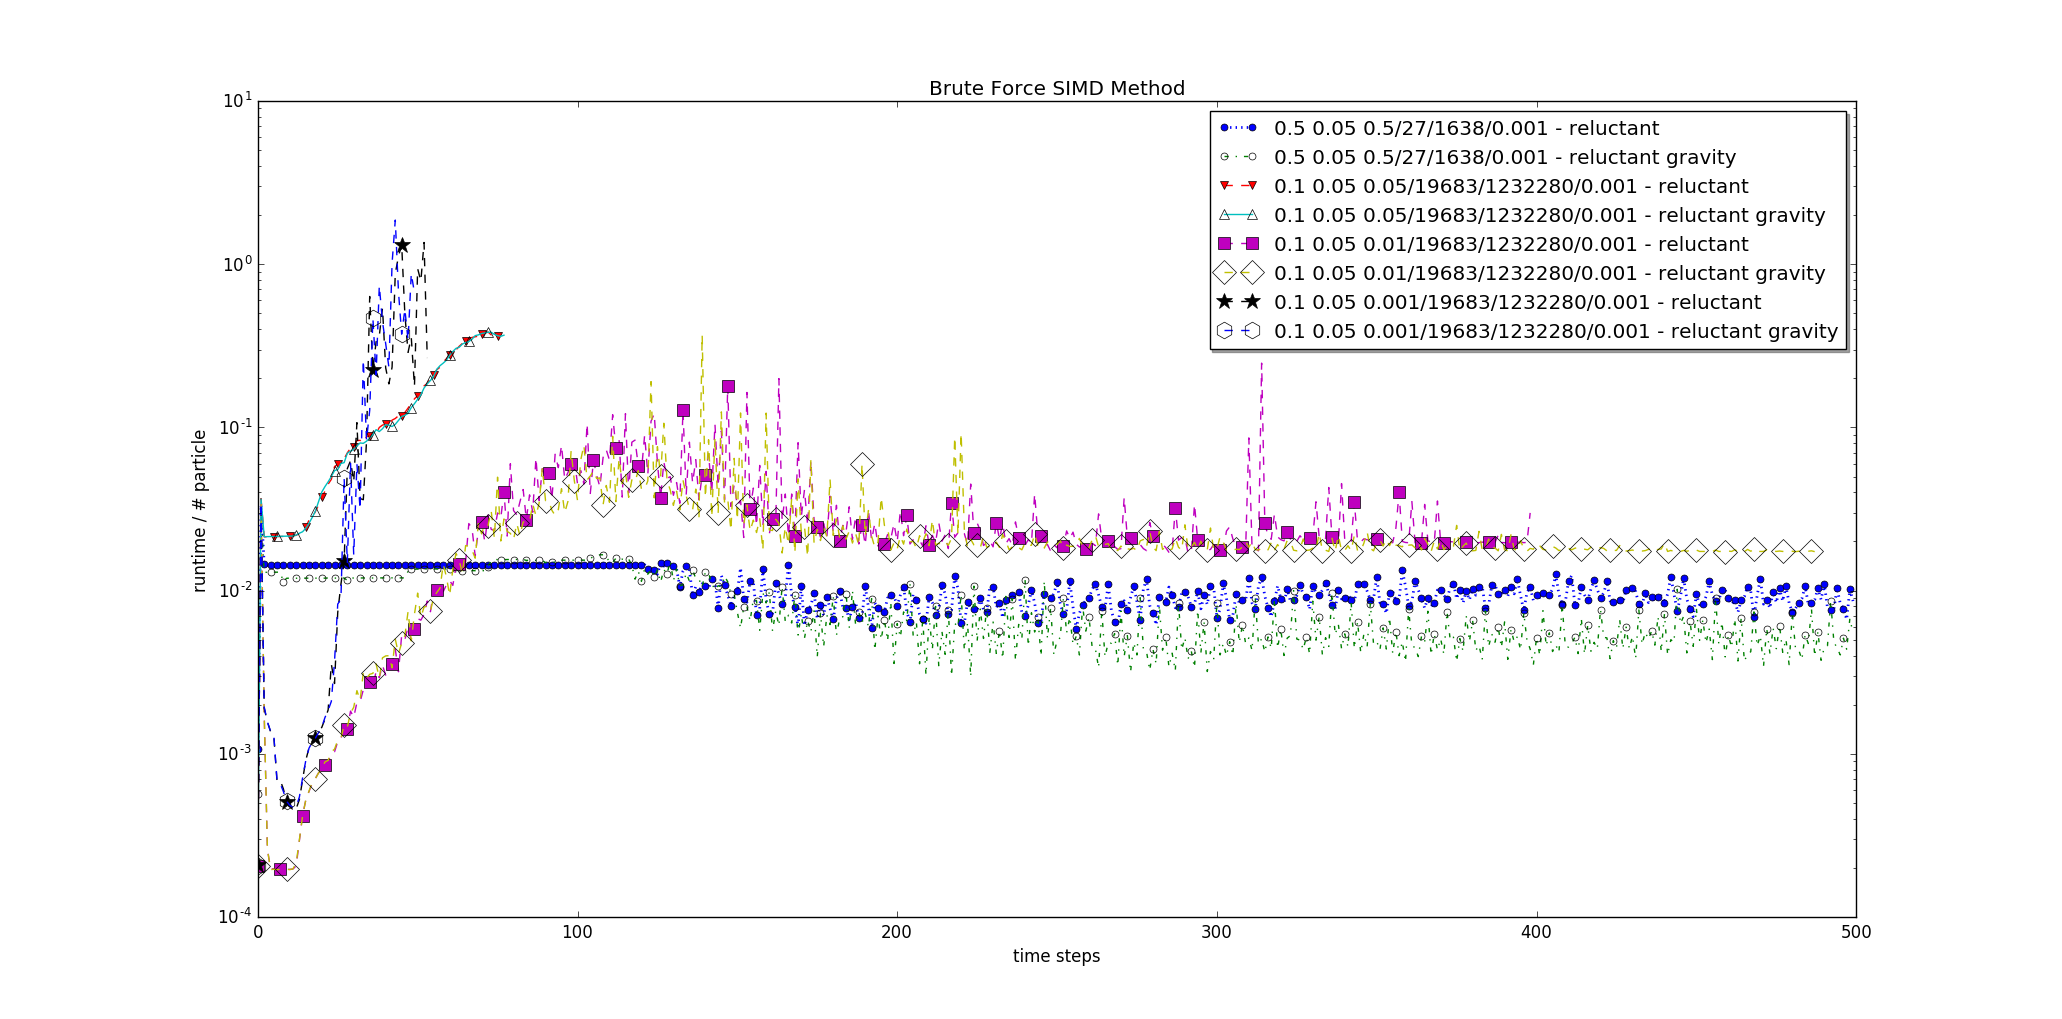
\includegraphics[width=1\textwidth]{experiments/vectorisation/plots/log_bf_simd.png}
  \end{center}
  \caption{Brute Force SIMD runtimes.}
  \label{figure:triangle_omp}
\end{figure}


penalty vectorization

\begin{figure}[htb]
  \begin{center}
    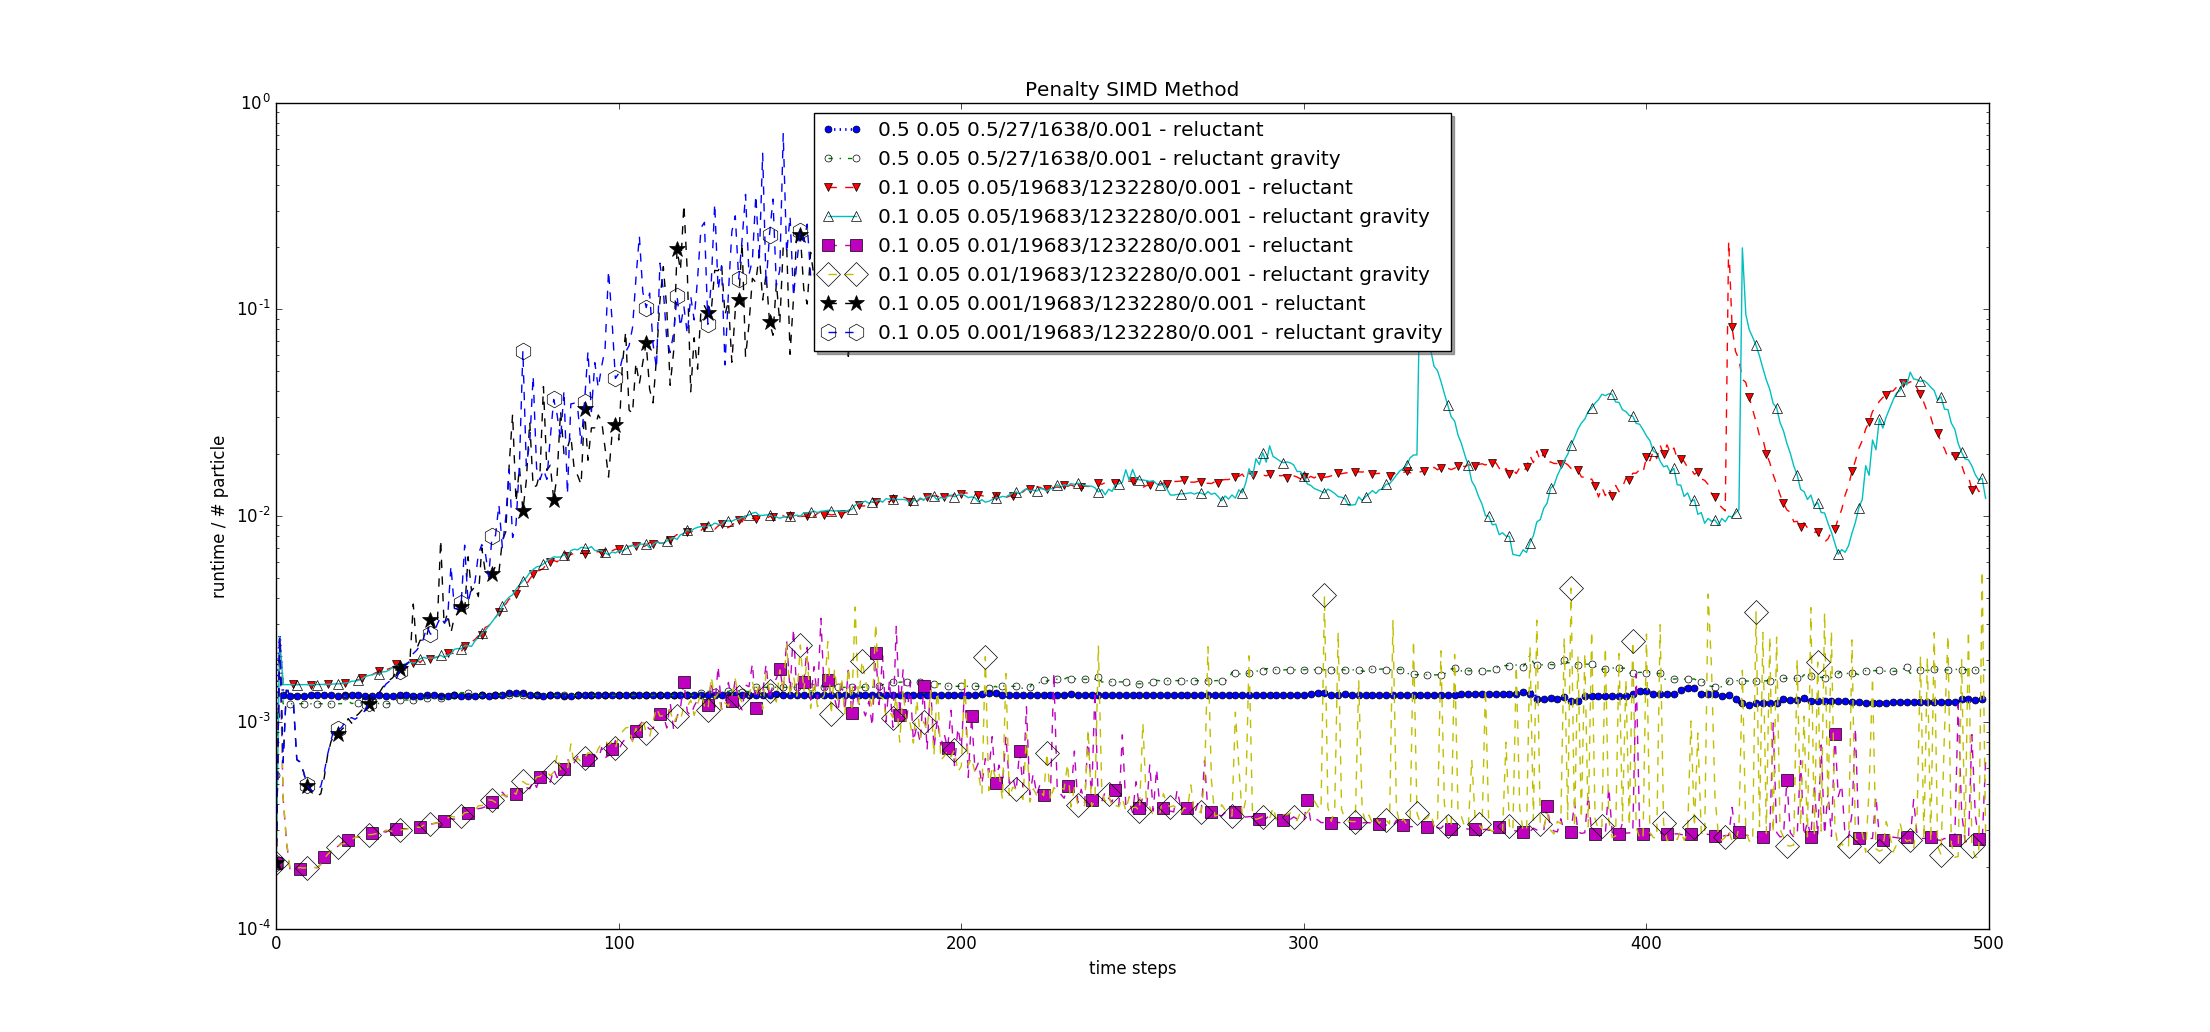
\includegraphics[width=1\textwidth]{experiments/vectorisation/plots/log_penalty_simd.png}
  \end{center}
  \caption{Penalty SIMD runtimes.}
  \label{figure:triangle_omp}
\end{figure}

hybrid vectorization

\begin{figure}[htb]
  \begin{center}
    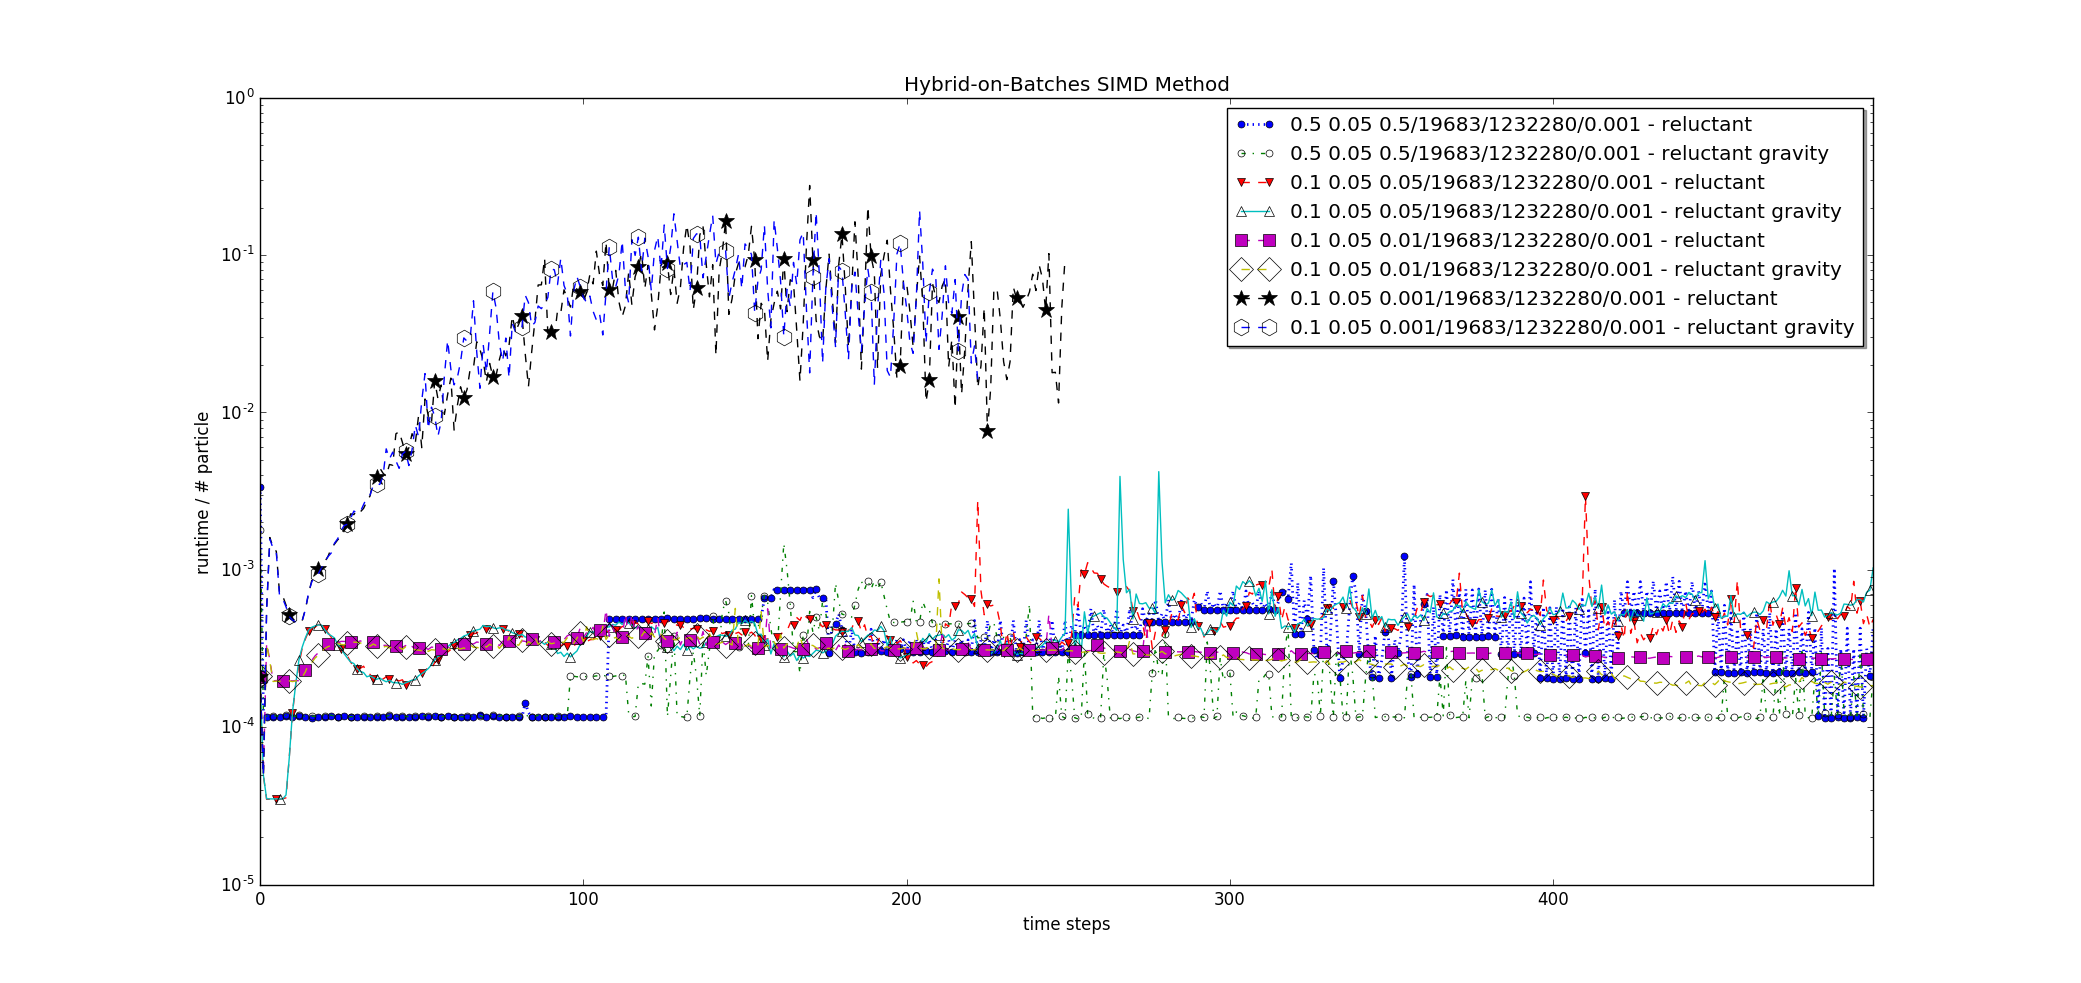
\includegraphics[width=1\textwidth]{experiments/vectorisation/plots/log_sphere-hybrid-on-batchesSIMD.png}
  \end{center}
  \caption{Hybrid-on-batches SIMD runtimes.}
  \label{figure:triangle_omp}
\end{figure}


\begin{figure}[htb]
  \begin{center}
    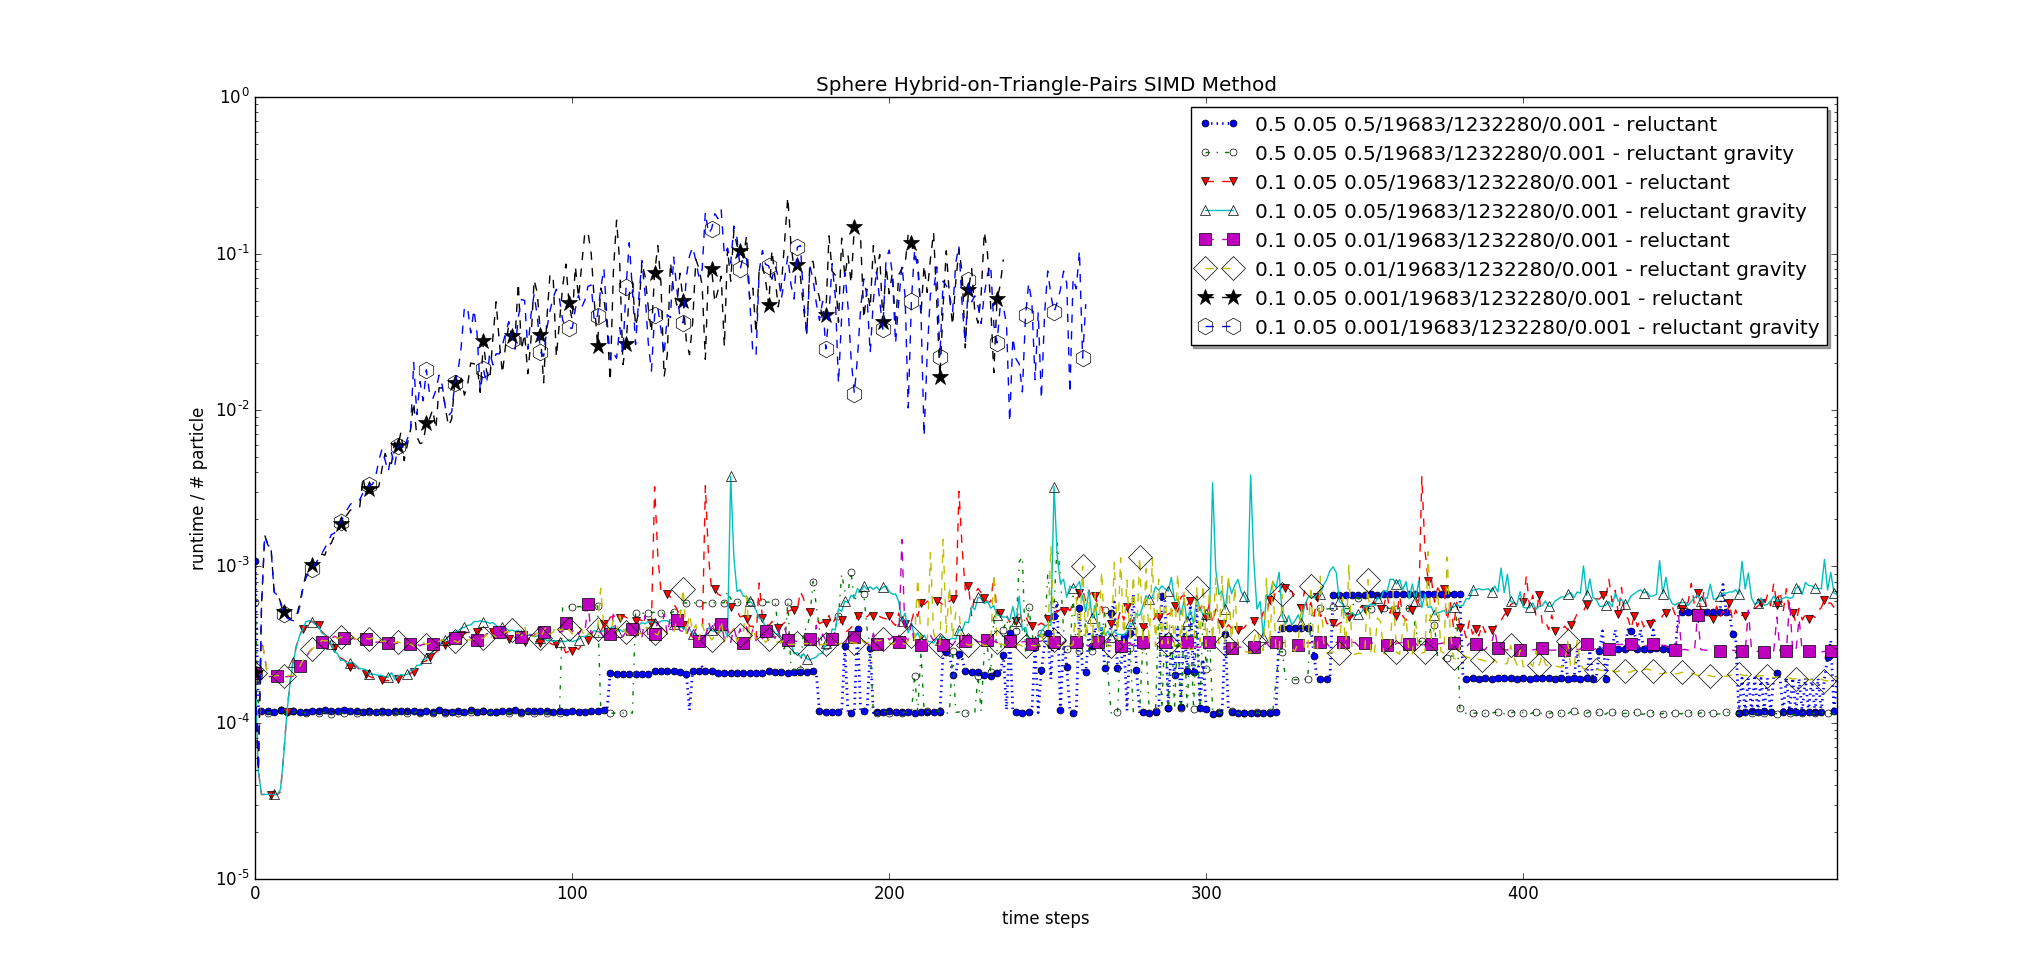
\includegraphics[width=1\textwidth]{experiments/vectorisation/plots/log_sphere-hybrid-triangle-pairs-SIMD.png}
  \end{center}
  \caption{Hybrid-on-triangle-pairs SIMD runtimes.}
  \label{figure:triangle_omp}
\end{figure}

overall vectorization speedup
\begin{figure}[htb]
  \begin{center}
    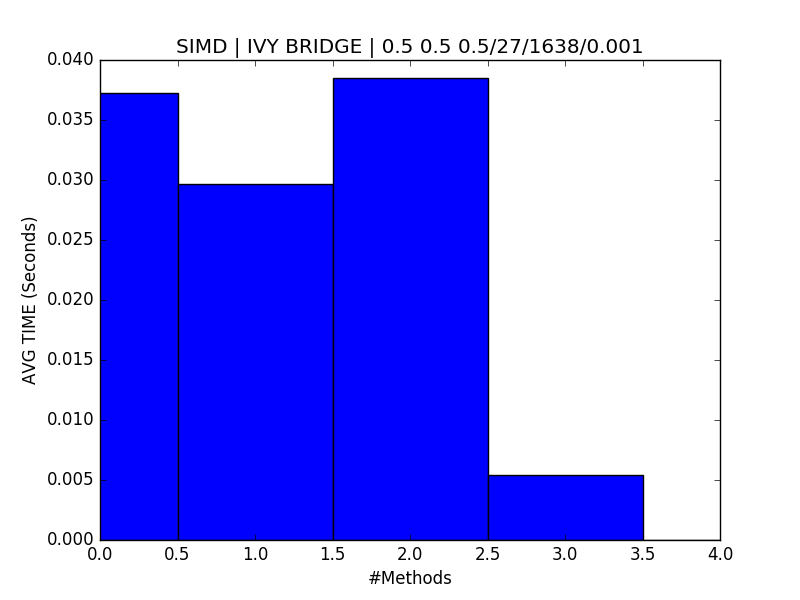
\includegraphics[width=1\textwidth]{experiments/vectorisation/plots/simd.png}
  \end{center}
  \caption{SIMD runtime comparison.}
  \label{figure:triangle_omp}
\end{figure}

\begin{figure}[htb]
  \begin{center}
    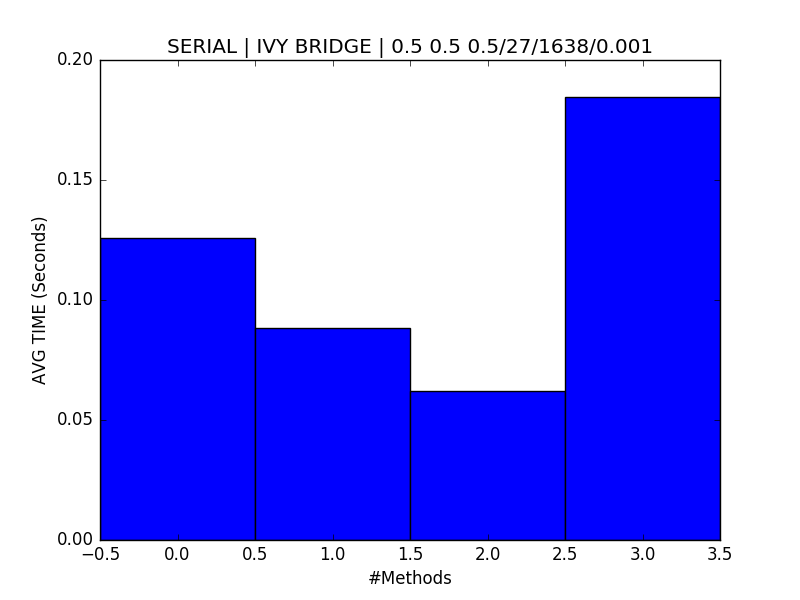
\includegraphics[width=1\textwidth]{experiments/vectorisation/plots/serial.png}
  \end{center}
  \caption{Serial runtime comparison.}
  \label{figure:triangle_omp}
\end{figure}


\clearpage

\subsection{Impact of multiscale grid management}

We start with single core experiments and $diam_{min} = diam_{max} \leq
h_{max}$ where $h_{max}$ is the grid spacing of a regular grid.
Alternatively, we remove the grid completely.
The number of triangle-to-triangle comparisons is reduced dramatically by the
grid which reduces the runtime complexity (Figure \ref{xxx}).
Runtime measurements reflect this fact directly (not shown).
If we release the equality constraint, select $diam_{min} < diam_{max}$ and
allow particles to have an arbitrary diameter between $diam_{min}$ and
$diam_{max}$, we retain the performance compared to the grid-free method.
Once we however use a dynamically adaptive multiresolution grid with inter-grid
particle comparisons, we can reduce the number of triangle-to-triangle
comparisons further. 
From hereon, the characteristic triangle-to-triangle comparison counts from the
multiscale algorithm are used.
For the performance engineering, this is a worst-case choice as the arithmetic
work is minimalised.



Cost
Cache hit rate
Stress on memory subsystem
